The increasing interest in lithium-ion batteries stems from their potential to offer efficient energy storage and contribute to environmental sustainability. Not only are LIBs widely employed in portable electronics like computers and cell phones, but they have also become integral to the power systems of electric and hybrid vehicles. The increasing popularity of LIBs in these applications can be attributed to their outstanding performance and high energy density \cite{kang2020binder}. Moreover, LIBs dominate the battery market for portable electronics, owing to inherent advantages such as high specific capacity and voltage, absence of memory effect, excellent cycling performance, minimal self-discharge, and a wide temperature range of operation \cite{zubi2018lithium}.

\vspace{5mm}

\begin{table}[ht]
    \centering
    \begin{footnotesize}
        \begin{tabular}{|p{7mm} p{22mm} p{113mm}|}
            \hline
            \rowcolor{bluepoli!40}
            \textbf{No.} & \textbf{Date} & \textbf{Accidents Replay}\T\B \\
            \hline \hline

            1 & Mar 2010 & Two iPod Nano music players overheated and caught fire, Japan\T\B\\

            2 & Apr 2010 & Acer recalled 2700 laptop batteries, as Dell, Apple, Toshiba, Lenovo and Sony did in 2006\T\B\\

            3 & Apr 2011 & EV taxi caught fire, Hangzhou, China\T\B\\

            4 & Jan-Dec 2013 & Three fire accidents of Boeing 747, happened in Boston America, Takamatsu, Tokyo Japan, respectively\T\B\\

            5 & Oct-Nov 2013 & 6 Tesla Model S EV cars caught fire\T\B\\

            6 & Apr 2015 & EV bus caught fire during charge, Shenzhen, China\T\B\\

            7 & May 2016 & The storage room of the LIB caught explosion, Jiangsu, China\T\B\\

            8 & Aug 2016 & Samsung Note 7 smart phone explosion\T\B\\

            9 & May 2017 & Panasonic announced to recall over 270 thousand LIBs\T\B\\

            10 & Oct 2017 & EV car caught fire, Austria\T\B\\

            11 & Jan 2018 & Tesla Model S EV car self-ignited, China\T\B\\

            12 & Jul 2018 & 4 MW/12 MWh energy storage system (ESS) caught fire and explosion, Korea\T\B\\

            13 & Jul 2018 & Electric scooter caught fire and explosion during charging, China\T\B\\
            \hline
        \end{tabular}
        \\[10pt]
        \caption[Lithium-ion battery accidents]{Lithium-ion battery fire and explosion accidents in the past few years. Source: Wang (2019) \cite{wang2019review}.}
        \label{table:accidents}
    \end{footnotesize}
\end{table}


Despite these merits, the broader expansion of the LIB market, especially in electric vehicles, faces significant challenges due to safety concerns \cite{love2018innovating,schipper2016recent,feng2018thermal}. Recent years have witnessed numerous recalls of LIBs, prompted by incidents of explosions and fires (Table \ref{table:accidents}), leading to substantial economic repercussions in related market sectors and tarnishing the reputation of LIBs \cite{chen2021review,balakrishnan2006safety}. As a result, there is a growing emphasis on addressing LIB safety issues, with the development of numerous safety strategies aimed at mitigating the risks associated with these batteries.

\section{Thermal Runaway}
\label{sec:thermal-runaway}

Even under normal operating conditions, battery-generated heat cannot be entirely removed. Rising battery temperature would trigger undesirable parasitic reactions, causing thermal runaway, where battery heat generation cannot be controlled \cite{wang2012thermal}.

Generally, thermal runaway occurs when the heat generated by exothermic reactions is not offset by the heat losses to the environment. This accumulated heat drives the temperature increase which, in turn, produces an exponential increase in the reaction rates. If the rate of heat generation exceeds the rate of heat dissipation into the environment, the temperature will continue rising. When reaching some critical temperatures, especially the collapse temperature of separator, the cell will breakdown.

\subsection{Causes for Thermal Runaway}
In the normal voltage and temperature range, only Li$^+$ shuttle occurs in the electrolyte during the insertion/extraction cycles at the cathode and anode. At high-temperature and high-voltage conditions, the electrochemical reactions become more complex, including decomposition of the solid electrolyte interface (SEI) film, oxygen release at the cathode side, and additional electrolyte/electrode parasitic side reactions \cite{maleki1999thermal}. SEI film decomposition and interfacial reactions initially accelerate the temperature increase, thereby increasing risks of oxygen release from the active cathode materials. These reactions eventually lead to LIB thermal runaway, which causes battery rupture and explosion due to the reaction of hot flammable gases from the battery with the ambient oxygen \cite{finegan2016investigating}.

During mechanical (damage to shell casing, compression, punching, and twisting of cells), electrical (overcharge/discharge and short circuit), and thermal abuse (thermal shock and local heating) situations, which could occur during accidents, thermal runaway will occur even quicker \cite{guo2010three,kim2007three,lamb2014evaluation}.
\vspace{5mm}

Figure \ref{fig:tr-graph} shows the origins of thermal runaway in LIBs, including side reactions of electrolyte, cathode, anode, and interfacial reactions at the surface of electrodes and Li plating. These side reactions are triggered by mechanical, thermal, and electrical abuse. Breakage of the separator and the oxygen evolution from the cathode side are the root causes to batteries' thermal runaway (as shown in the solid lines of Figure \ref{fig:tr-graph}d).

\begin{figure}[ht]
    \centering
    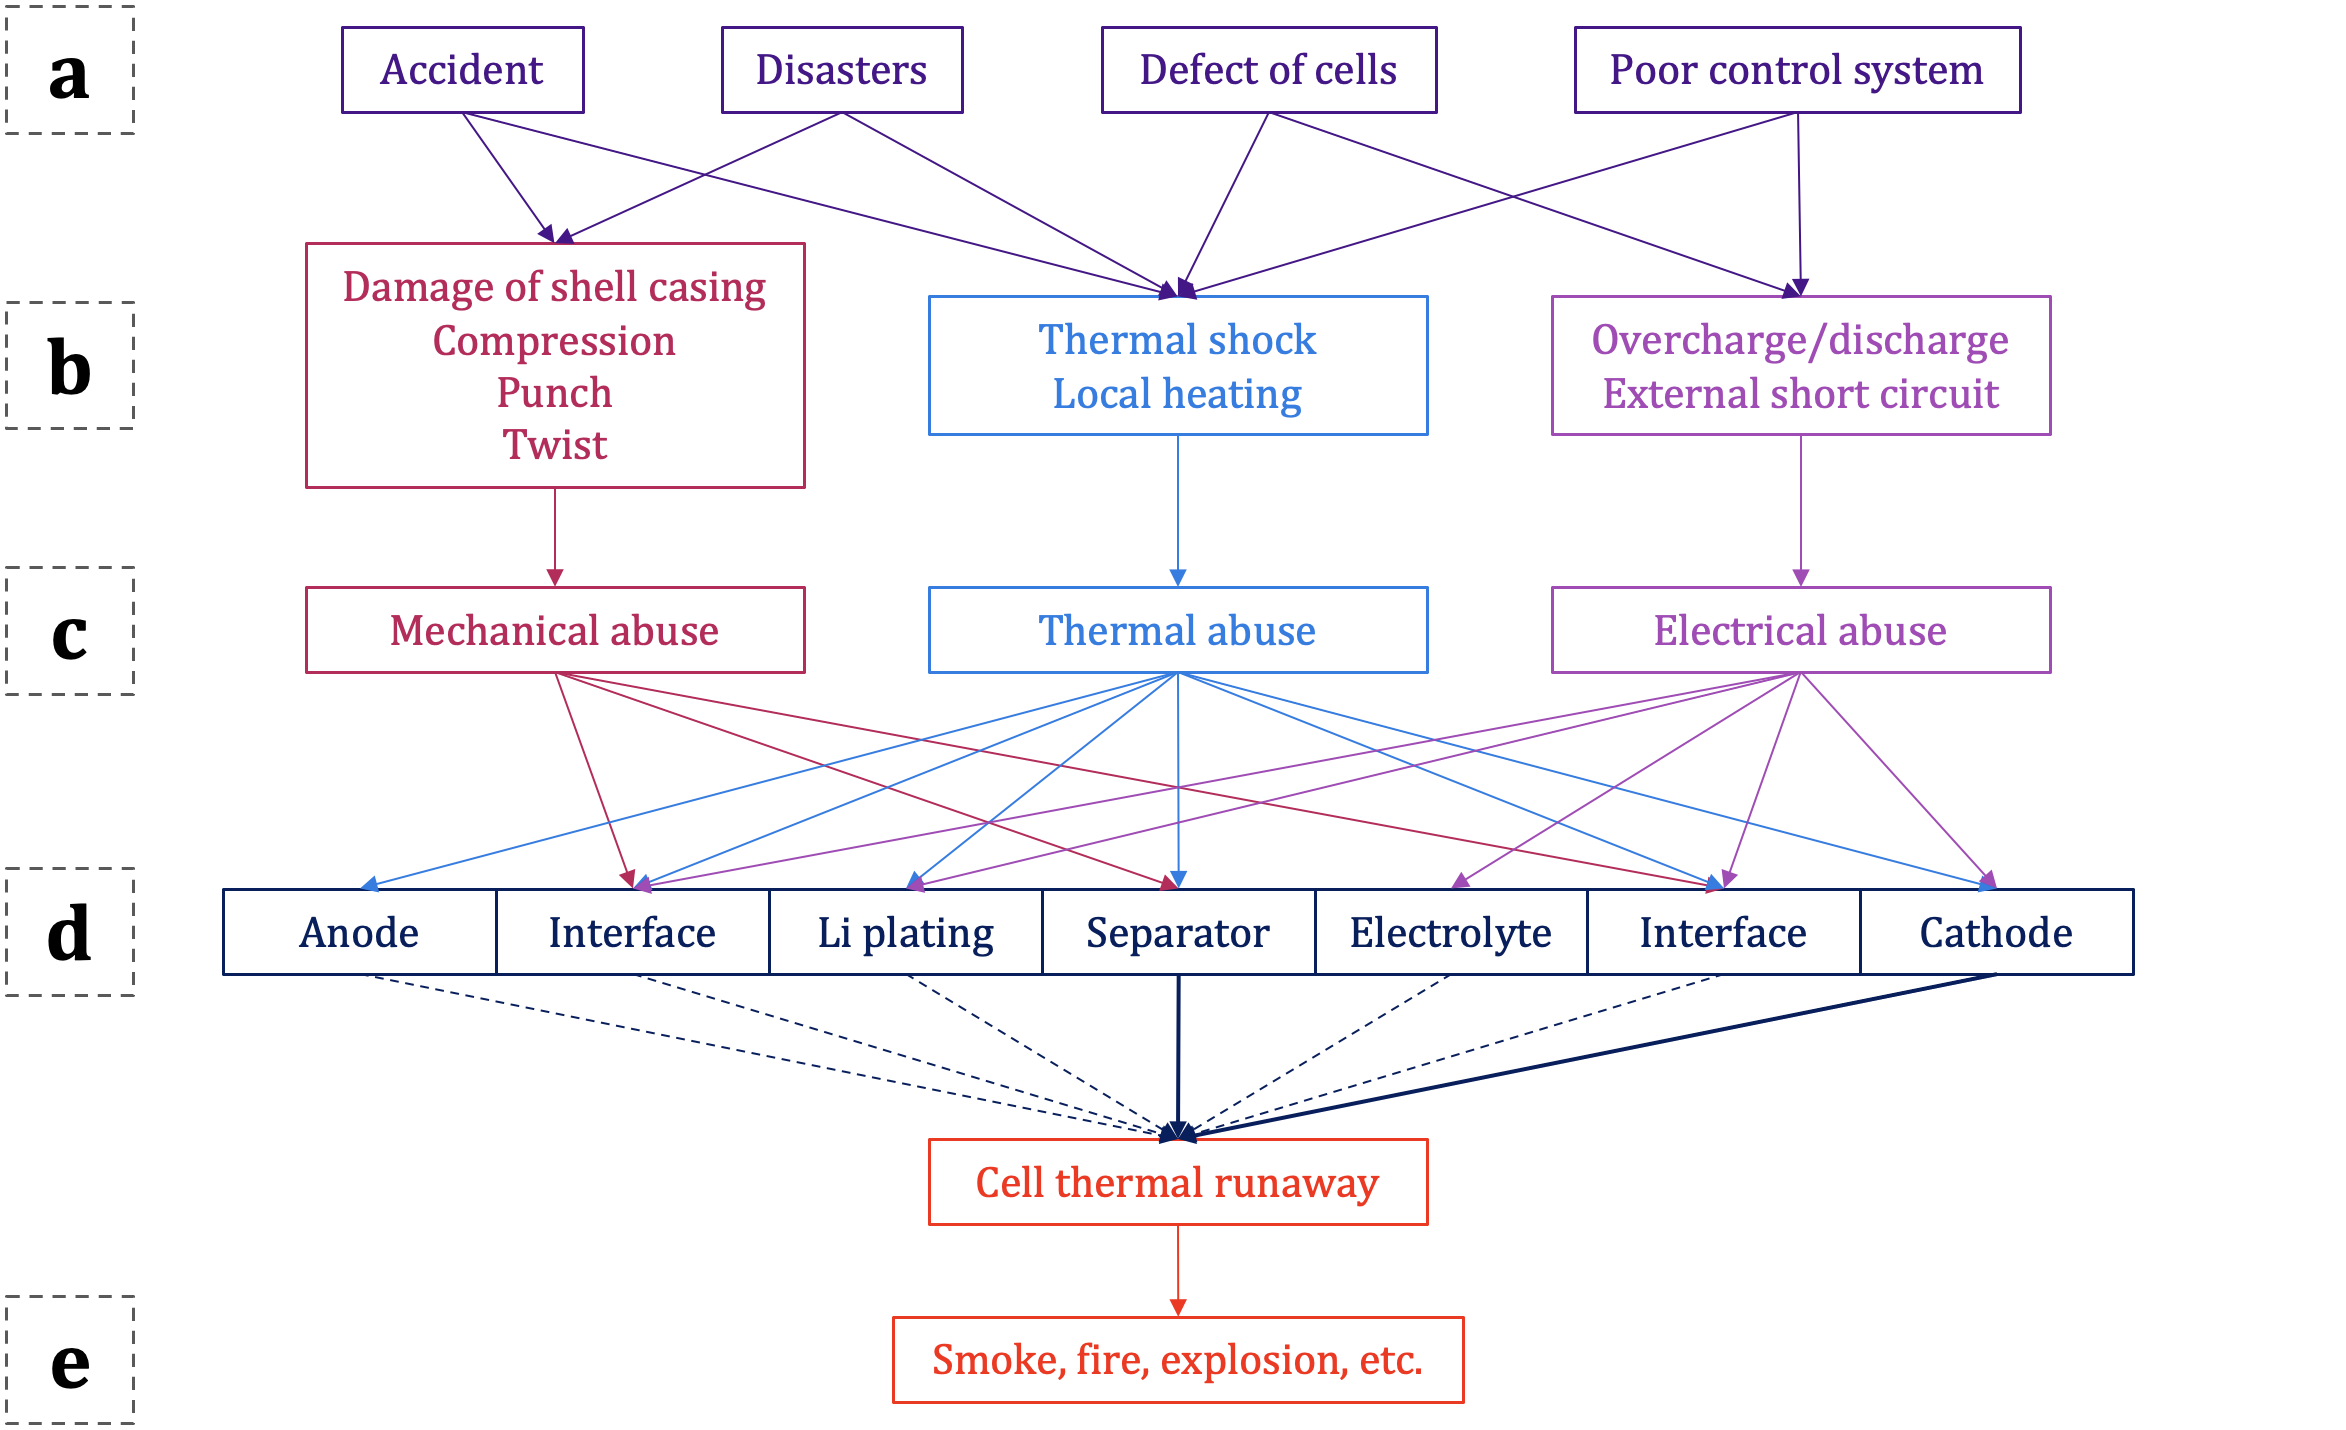
\includegraphics[width=0.9\textwidth]{Images/Chapter2/tr-graph.png}
    \caption[Schematic of the causes of lithium-ion battery thermal runaway]{Schematic of the causes of LIBs thermal runaway. Source: Chen (2020) \cite{chen2021review}.}
    \label{fig:tr-graph}
\end{figure}

The five types of causes for thermal runaway are listed below.
\begin{enumerate}
    \item \textbf{Uncontrollable internal heat generation} causes oxygen release from the cathode material, leading to numerous side reactions \cite{jung2017oxygen};
    \item \textbf{Separator defects} (due to thermally-induced shrinkage or mechanical damage) create short circuits in the battery and rapid discharge of the energy stored in it, accompanied by undesirable chemical chain reactions and release of massive amounts of heat \cite{wang2015alumina};
    \item \textbf{Electrical abuse}, especially in a high state of charge, causes electrolyte decomposition at the cathode interface. This leads to heat accumulation and consequently release of oxygen from the cathode and damage to the separator \cite{ren2017electrochemical};
    \item \textbf{Thermal abuse} gives rise to electrochemical side reactions and heat generation. If the heat cannot be dissipated quickly enough, the separator will shrink or rupture \cite{tarascon2001issues,kim2014shape};
    \item \textbf{Mechanical abuse} causes short circuits and/or air to penetrate the battery, originating a failure \cite{liu2020safety}.
\end{enumerate}

\subsection{Semenov Model}
\label{sec:semenov-model}
The Semenov plots \cite{semenov2013some} shown in Figure \ref{fig:semenov-plot} can be used to further illustrate the dynamics of the thermal runaway. The curved line (line 4) represents the heat generation due to the exothermic reaction (exponential function, following the Arrhenius law), while the straight lines 1, 2 and 3 represent the heat loss under different ambient temperatures (ambient temperature $A$, $B$ and $C$, respectively) which is a linear function following the Newton's law of cooling. 

\begin{figure}[ht]
    \centering
    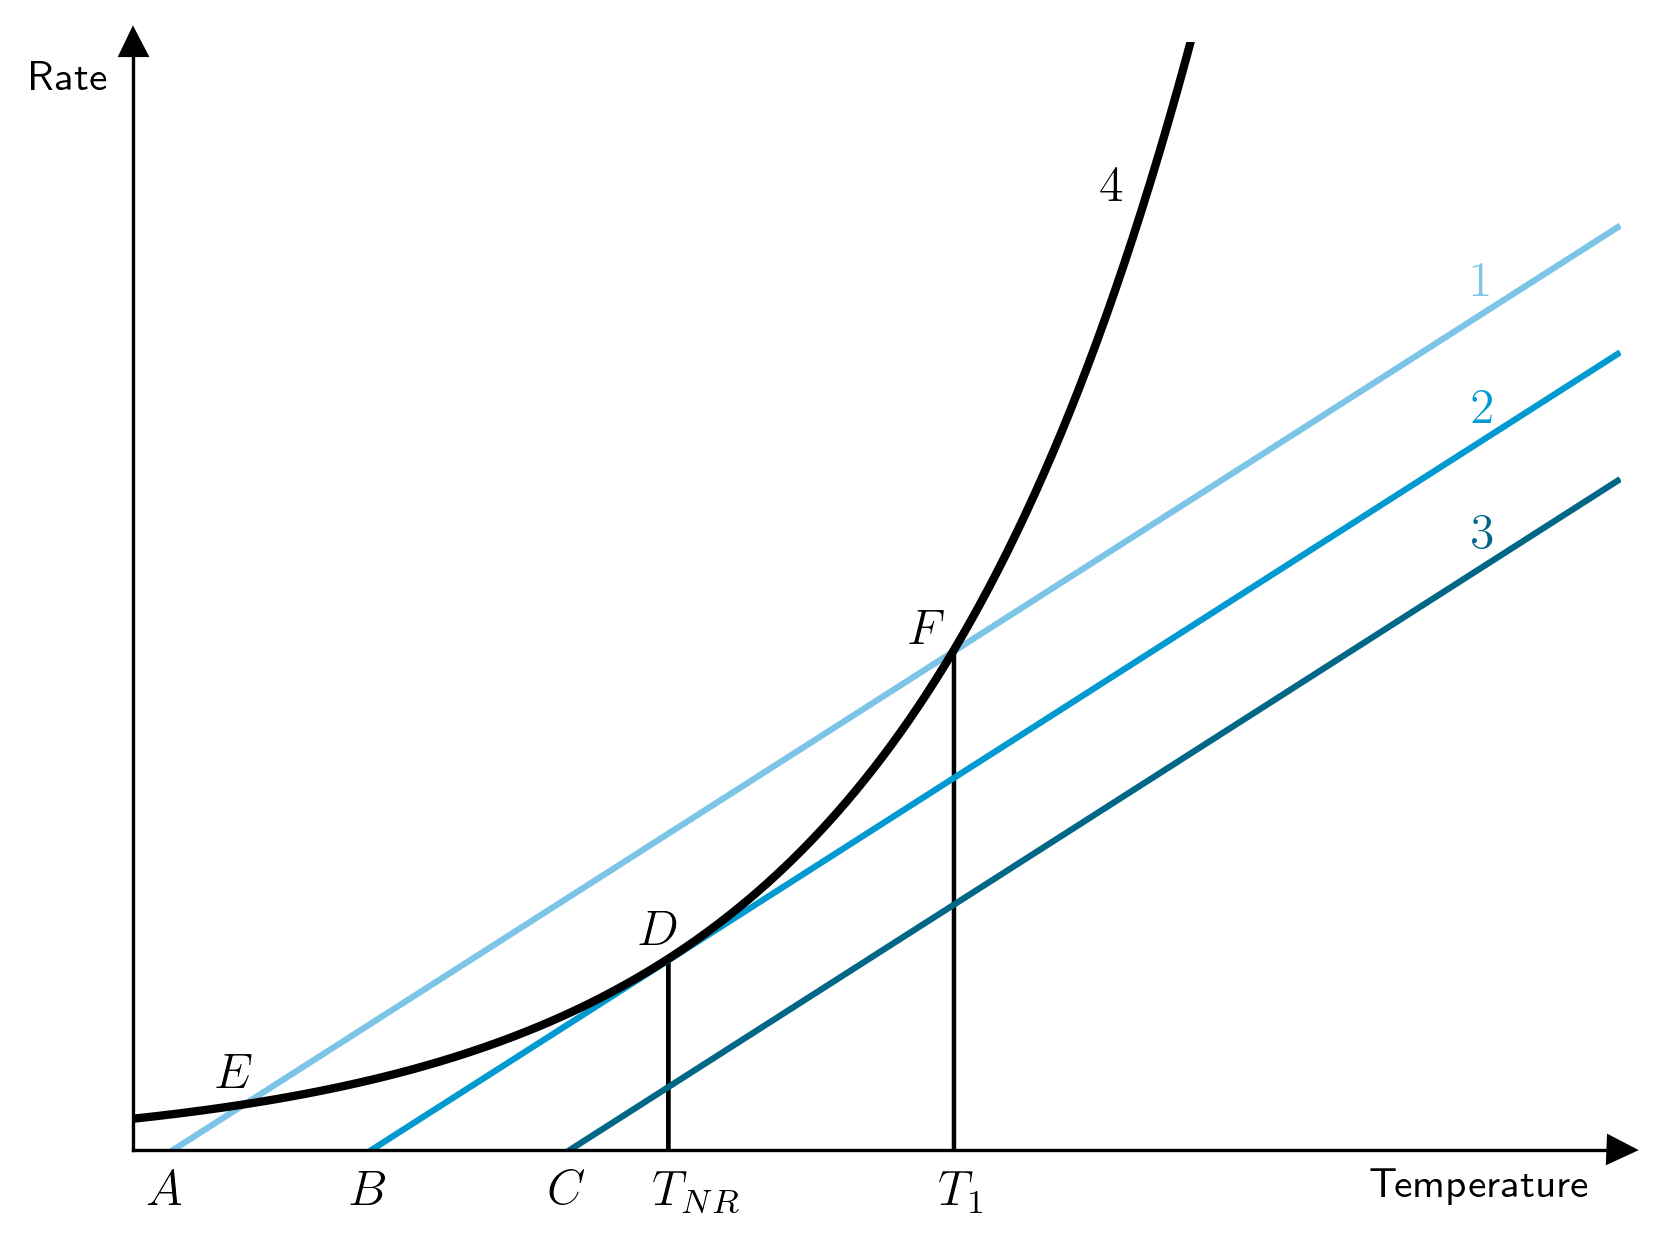
\includegraphics[width=0.7\textwidth]{Images/Chapter2/semenov-plot.png}
    \caption[Temperature dependence of reaction rate and heat loss]{Temperature dependence of reaction rate and heat loss from a system at three ambient temperature: $A$, $B$ and $C$. Source: Semenov (2013) \cite{semenov2013some}.}
    \label{fig:semenov-plot}
\end{figure}

When the ambient temperature is $A$, there are two intersection points ($E$, $F$) between line 4 and 1, where the heat generation rate is equal to the heat loss rate. The lower point E is a stable thermal balance point. If temperature deviates upwards, the cooling rate is higher than the heat generation rate, so the system will return to point $E$. If temperature drops, the heat generation rate is higher than the cooling rate, so the system will return to point $E$ again. Point $F$ is an unstable and also an unreachable point, because the heat loss rate is higher than the heat generation rate before $T_1$ , so the system will cool to point $E$ rather than heat to point $F$. When the ambient temperature increases to $B$, line 2 has one tangent point $D$ with line 4. At this point, the heat loss rate is equal to the heat generation rate, and once the system temperature increases a little, the system's temperature will continue to rise at a progressively higher rate. This critical equilibrium temperature is called the “Temperature of No Return, $T_{NR}$ ”, and the ambient temperature $B$ is the self-accelerating decomposition temperature (SADT). LIB can be regarded as a reaction system, in which the heat comes from the electrochemical reactions between its components.

Semenov plots illustrate only a special case for LIB thermal runaway rather than a universal model. In the realistic reaction process, the system is hard to reach uniform temperature distribution, but Semenov model can simplify
the problem. In fact, many realistic situations could be solved based on the assumption of uniform temperature distribution. Many investigators still assumed that the temperature inside the battery was spatially uniform before thermal runaway in external heating and self-heating test \cite{liu2015comprehensive,feng2014thermal}.

\subsection{Energy Balance}
\label{sec:energy-balance}
Questa parte si può prendere pari pari da "Thermal runaway - 2565" pagine 4-5. Inoltre si può prendere qualcosa anche da "Failure description - 43" (anche qua descrizione dei failure modes component-wise con bei grafichini) e da "Failure description - 890".

\subsection{Basic Reactions}
\label{sec:basic-reactions}
\begin{table}[ht]
    \centering
    \begin{footnotesize}
        \begin{tabular}{|P{55mm} P{28mm} P{20mm}|}
            \hline
            \rowcolor{bluepoli!40}
            \vspace{0.1mm}\textbf{Reactions} & \textbf{Temperature range [$^\circ$C]} & \textbf{Enthalpy [J/g]}\T\B \\
            \hline \hline

            SEI decomposition & 100-130 & 186-257\T\B\\

            LiC$_6$/electrolyte & 110-290 & 1460-1714\T\B\\

            LiC$_6$/PVDF & 220-400 & 1100-1500\T\B\\

            Li$_x$CoO$_2$ decomposition & 178-250 & 146\T\B\\

            Li$_x$Ni$_{0.8}$Co$_{0.2}$O$_2$ decomposition & 175-340 & 115\T\B\\

            Li$_x$CoO$_2$/electrolyte & 167-300 & 381-625\T\B\\

            Li$_x$Ni$_{0.8}$Co$_{0.2}$O$_2$/electrolyte & 180-230 & 600-1256\T\B\\

            Electrolyte decomposition & 225-300 & 155-258\T\B\\
            \hline
        \end{tabular}
        \\[10pt]
        \caption[Exothermic reactions occurring in LIBs]{Temperature ranges and enthalpies of various exothermic reactions occurring in LIBs. Source: Chen (2021) \cite{chen2021review}.}
        \label{table:reactions}
    \end{footnotesize}
\end{table}



\section{Safety Standards}
\label{sec:safety-standards}
Safety standards and corresponding assessments have been established to analyze battery performance and key factors, aligning with the necessary safety requisites. The stringent and rigorous battery safety tests are designed to minimize the likelihood of safety issues in routine working conditions and ensure that batteries available on the market are of sufficient quality for intended purposes. Thanks to these measures, contemporary LIBs exhibit a significantly enhanced safety profile compared to their predecessors. Nonetheless, ongoing advancements are imperative to further improve battery safety standards \cite{chen2021review}.

Hence, various international organizations regulate battery safety, and governments of different countries have formulated standards in accordance with national requirements and conditions and have gradually improved the safety standards of lithium-ion batteries. Academics and industrial groups have also carried out extensive research on battery safety.

Most countries and international organizations have developed LIB safety oriented standards, which include:
\begin{enumerate}
    \item Chinese standard GB/T 31485 \cite{GBT31485};
    \item Society of Automotive Engineers (SAE) standard 2464 \cite{SAE2464};
    \item International Electrotechnical Commission (IEC) standard IEC62133 \cite{IEC62133-2};
    \item United Nations (UN) standard UN38.3 \cite{UN38.3};
    \item Japanese Industrial Standard (JIS) C8714 \cite{JISC8714};
    \item Underwriters Laboratories (UL) standard UL2580 \cite{UL2580};
    \item International Standardization Organization (ISO) standard ISO 16750-2 \cite{ISO16750-2:2023}.
\end{enumerate}

Since the various safety test standars apply different methodologies, a summary of some test requirements and comparisons of five test items are presented in Table \ref{table:standards}.

\begin{table}[ht]
    \centering
    \begin{scriptsize}
        \begin{tabular}{|P{20mm} P{29mm} P{29mm} P{29mm} P{29mm}|}
            \hline
            \rowcolor{bluepoli!40}
            & \textbf{GB/T31485} & \textbf{IEC62133} & \textbf{UL2580} & \textbf{SAE J2464}\T\B \\
            \hline \hline

            \textbf{Heating} & Heating at 5 $^\circ$C/min from 25 $^\circ$C to 130 $^\circ$C, hold for 30 mins \vspace{3mm}& 130 $^\circ$C, 10 mins & 150 $\pm$ 2 $^\circ$C, 60 mins & Max. stable temperature\T\B\\

            \textbf{Short-circuit} & Short circuit for 10 mins, $R\leq$ 5m$\Omega$ & 80$\pm$20m$\Omega$ & Short with $R\leq$ 5m$\Omega$ until explosion, fire or no temp change & $R\leq$ 5m$\Omega$ for hard short; $R\geq$ 5m$\Omega$ for soft short\vspace{3mm}\T\B\\

            \textbf{Overcharge} & 100\% SOC Overcharge to 1.5 $V_{max}$ or charge for 1 hour at 1C \vspace{3mm}& Overcharge to 250\% SOC at 1C & Overcharge to 200\% SOC at 1C & Overcharge to 200\% SOC at 1C\T\B\\

            \textbf{Over-discharge} & Over-discharge the 100\% SOC cell at 1C for 1.5 hours \vspace{3mm}& Over-discharge the 0\% SOC cell at 1C for 90 mins & Over-discharge the 0\% SOC cell at 1C for 90 mins & Over-discharge the cell to -100\% SOC\T\B\\

            \textbf{Nail penetration} & Penetration rate 25 mm/s, $\varphi$ 5$\sim$8mm, 100\% depth & / & 80 mm/s, $\varphi$ 3mm, 100\% depth & 80 mm/s, $\varphi$ 3mm, 100\% depth\T\B\\
            \hline
        \end{tabular}
        \\[10pt]
        \caption[Testing standards coparison]{Testing standards comparison of selected items. $\varphi$ represents the nail diameter. Source: Chen (2021) \cite{chen2021review}.}
        \label{table:standards}
    \end{scriptsize}
\end{table}

\subsection{Safety Tests}
\label{sec:safety-tests}
Analysis of the presence of various LIB defects and shortcomings can help to define specific LIB safety issues or hazards. Extensive testing uncovers these issues to assist efforts to ensure that future generations of batteries are safer and more reliable. In a safety test possible trigger modes are simplified so batteries thermal runaway characteristics are measurable in the laboratory. Laboratory environment test conditions must generally be more stringent than "real-world" conditions to ensure safety during actual use. For example, batteries being tested have to be maintained at a 100\% state of charge (SOC). The three principles of operability, repeatability and reproducibility should be met in the process of formulating a safety standard. 

Here follows a brief description of the main safety tests used to examine key LIB properties.

\subsubsection{Electrical Abuse Tests}
\label{sec:electrical-abuse-tests}
When a battery is in an overcharge or over-discharge state, or is undergoing a short circuit, it experiences electrical abuse, and a series of undesirable electrochemical reactions occurs in it.

There are many reasons for battery overcharging. One of the main reasons is the inconsistency of battery cells. If the voltage of any battery cell cannot be effectively monitored by the management system, there will be risks of its overcharging. Since excess energy is stored into the battery, overcharging is very dangerous.

\begin{figure}[ht]
    \centering
    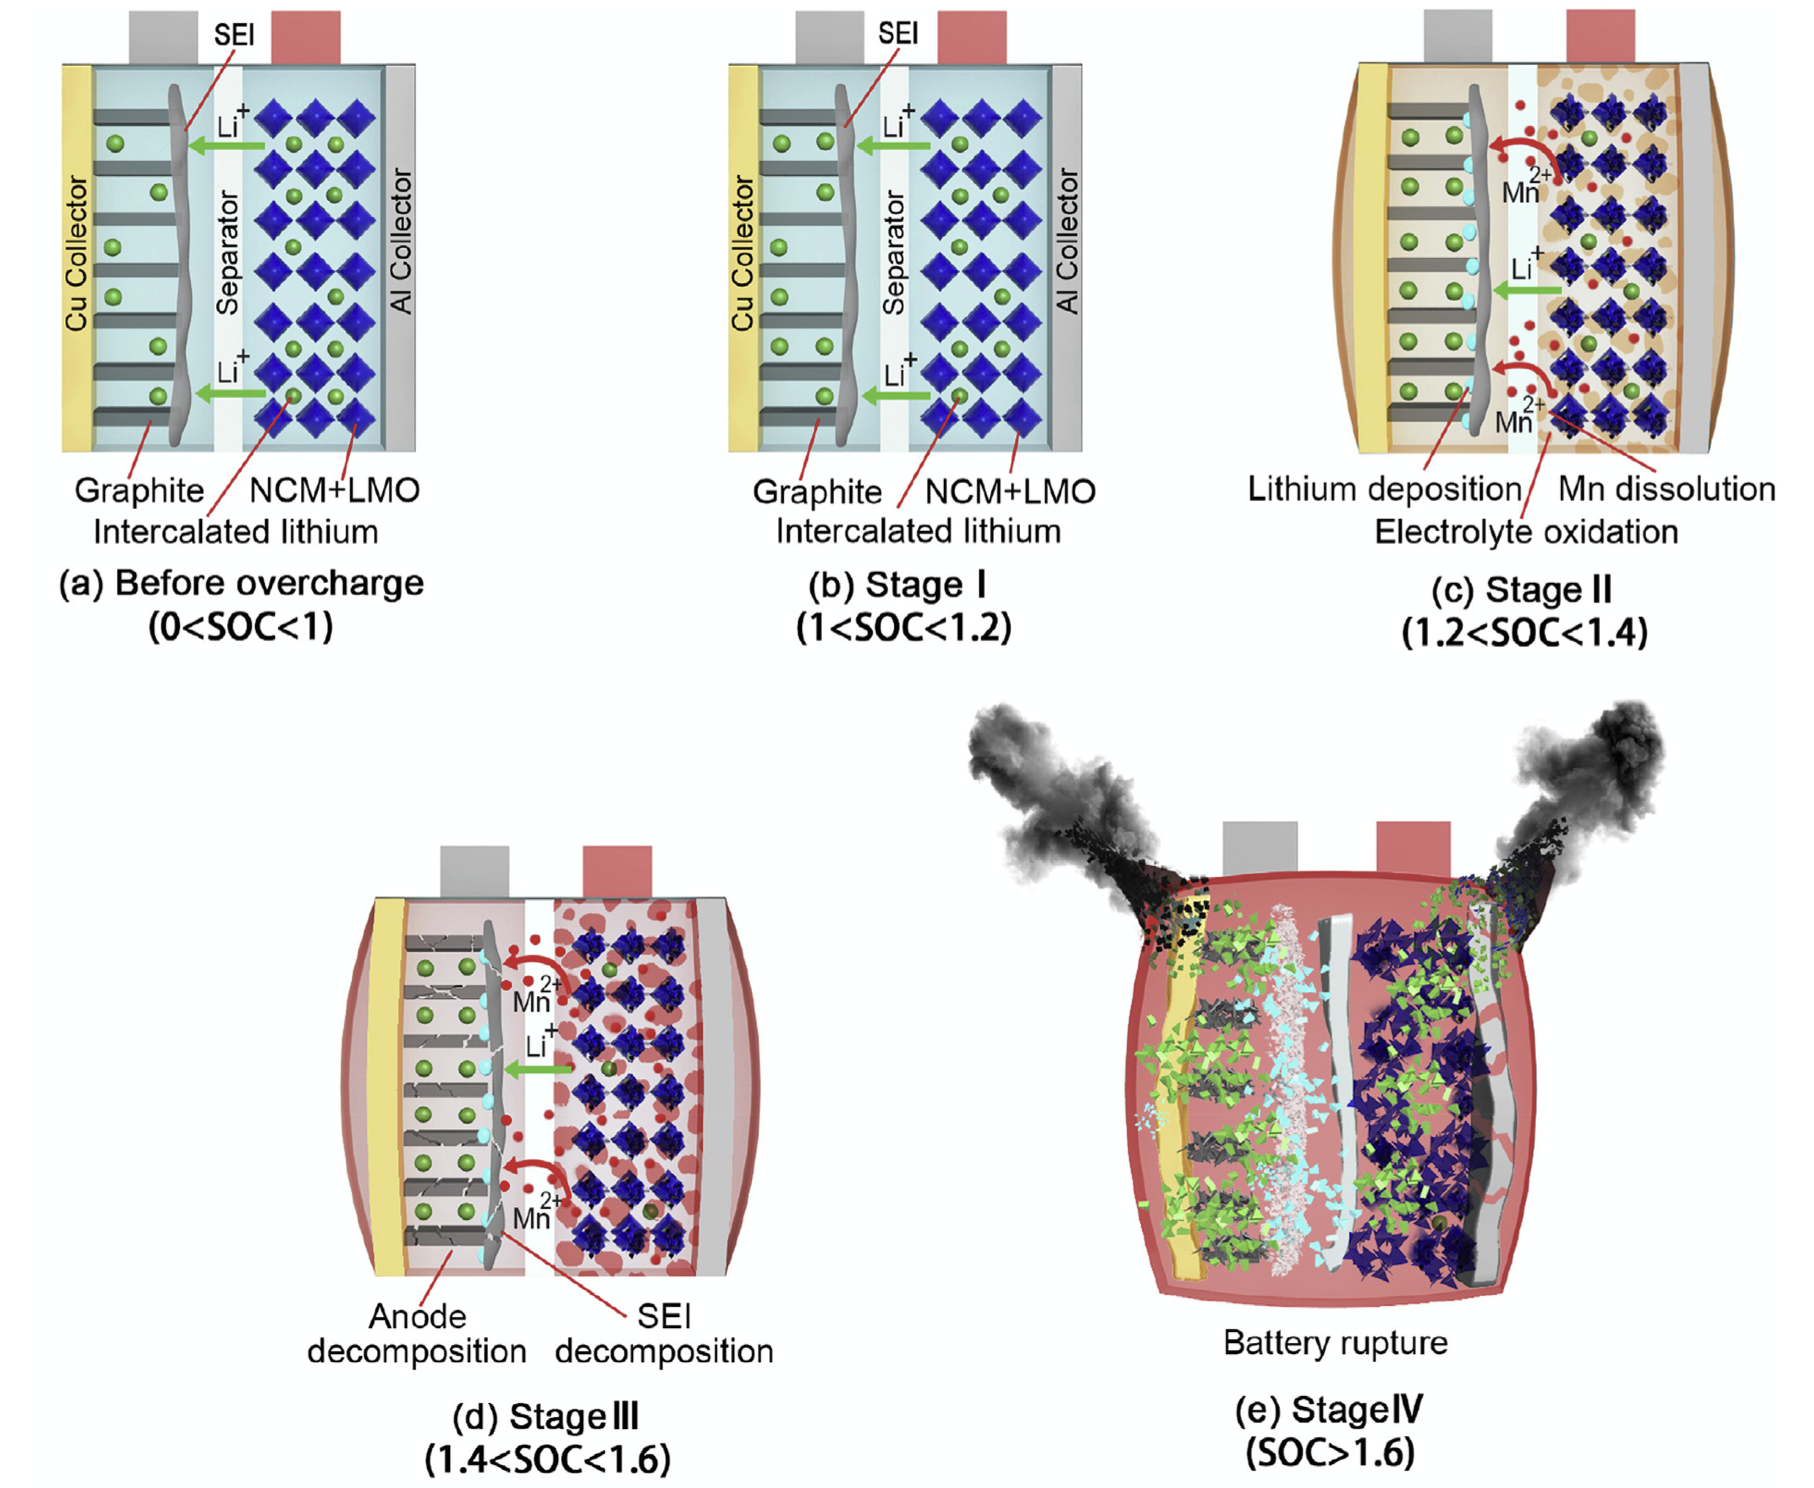
\includegraphics[width=0.8\textwidth]{Images/Chapter2/overcharge-failure.png}
    \caption[Overview of the overcharge side reactions]{Overview of the overcharge side reactions at each stage for lithium ion batteries with NCM + LMO cathode. Source: Ren (2017) \cite{ren2017electrochemical}.}
    \label{fig:overcharge-failure}
\end{figure}

Overcharge first causes electrolyte decomposition at the cathode interface \cite{ohsaki2005overcharge}. This reaction slowly increases the battery temperature. Subsequently, excessive Li+ deintercalation from the cathode occurs. The cathode material becomes unstable and start to release oxygen, while excess Li+ deposits on the anode to form Li dendrite \cite{arai2015situ}. Heat and gas generation during the side reactions would lead to safety accidents, such as cell overheating and rupture \cite{lisbona2011review}.

The principle of over-discharge is similar that of overcharge. Some cells reach the set state of discharge (SOD) in advance. Thus, an over-discharge occurs if a cell is forced to continue to discharge \cite{li2008effect}. Forced over-discharge continuously releases Li+ from the anode, which change the graphite structure and destroy the SEI. At very deep SOD, a copper current collector is oxidized, with the released copper ions potentially being deposited on the cathode surface \cite{ouyang2018investigation}. Too much copper deposition results in the short-circuit of cell.

\begin{itemize}
    \item \textbf{Overcharge/over-discharge tests} are intended to assess processes that occur in a cell when the charge or discharge processes are out of control. According to the IEC standard test, the cell is first discharged to 3.0 V, and then is charged under 10 V. If the battery does not combust or explode during or after the test it is considered safe, its materials (electrolyte, active electrode materials, separators etc.) are regarded as having adequate properties, and the structural design is deemed satisfactory. The safety performance under overcharge is closely related to the charge rate, so overcharging is performed at different rates to establish at which extreme rate and voltage failure occurs \cite{chen2021review}.
    \item \textbf{Internal short circuit (ISC) tests} assess the short circuiting that is caused by internal electrical connections of battery poles under abnormal conditions. Several methods are used to initiate an internal short circuit, including nail penetration, heavy impact, crush and forced ISC \cite{chen2021review}. 
    \item \textbf{External short circuit tests} assess the short circuiting that is caused by external electrical connections of battery poles under abnormal conditions. According to the GB31485-2015 procedure, the battery is kept at 25 $\pm$ 2 $^\circ$C in a fully charged state for 30 minutes, then the cathode and anode terminals are connected with a wire, and the external resistance is kept at 5 m$\Omega$. During this test, the temperature and voltage are monitored simultaneously, throughout the entire test. The test is considered successful if the cell does not explode or combust \cite{chen2021review}.
\end{itemize}

\subsubsection{Mechanical Abuse Tests}
\label{sec:mechanical-abuse-tests}
Due to the high energy density of LIBs, local damage caused by external influences, for example in case of collisions, will release a significant amount of heat, which can easily cause thermal runaway. As a result their safety risk is high. As the number of EVs (containing LIBs) on the roads continues to increase, safety concerns over battery behavior during potential vehicle collisions are becoming more prominent \cite{chen2021review}.

Mechanical abuse tests are conducted in order to assess LIB safety under mechanical abuse conditions (e.g. crushing, penetration, and vibration) that may occur during battery production, transportation, and use.

\begin{figure}[ht]
    \centering
    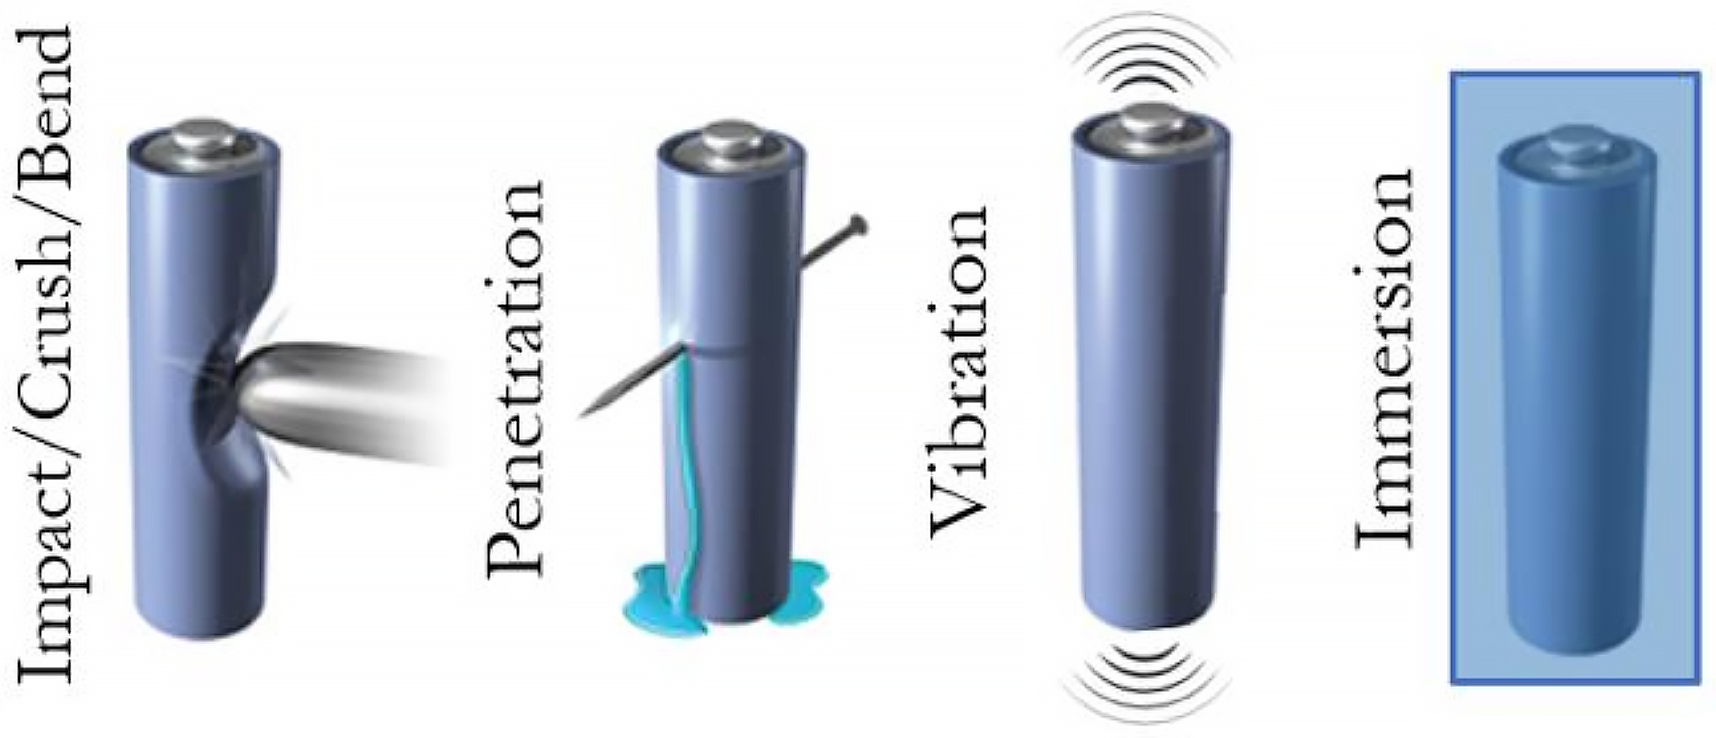
\includegraphics[width=0.6\textwidth]{Images/Chapter2/mechanical-failure.png}
    \caption[Illustration of various mechanical abuse mechanisms]{Illustration of various mechanical abuse mechanisms. Source: Fransson \cite{fransson2024phd}.}
    \label{fig:mechanical-failure}
\end{figure}

\textbf{Nail penetration tests} are the most common type of mechanical tests, and they are designed to simulate internal battery short circuits arising when a battery's internal membrane is penetrated by impurities. According to GB/T 31485, a fully-charged battery should be penetrated with a high temperature-resistant steel spike of $\varphi$ 5$\sim$8 mm in a direction perpendicular to the polar plate at a speed of 25 $\pm$ 5 mm/s. The penetration position should also be close to the geometric center of the penetrated surface, with the steel spike retained inside the battery. The test is considered successful if the cell does not explode or combust \cite{chen2021review}.

\subsubsection{Thermal Abuse Tests}
\label{sec:thermal-abuse-tests}
In thermal abuse situations, a battery experiences thermal shock, or its local temperature is too high \cite{wang2019thermal}. In theory, battery cycling cannot cause safety accidents because the heat generated during normal anodic and cathodic reactions is insufficient to cause a sharp temperature increase. In reality, however, the electrode heat release rate is often higher than its cooling rate. Heat dissipation of a LIB depends on its external surface area and geometry. Heat dissipation by radiation helps to alleviate some of the generated heat. As a result, some of the heat remains stored inside the battery. At some point, if this heat continues to accumulate instead of being dissipated, exothermic side reactions start to occur, further concentrating thermal stress \cite{bandhauer2011critical}.

\textbf{Heating tests} assess the thermal runaway caused by a battery being heated due to local overheating, and the subsequent thermal runaway expansion. Heating is used to analyze LIBs' thermal stability and heat distribution to ensure they have sufficiently efficient heat management and capability to forecast potential hazards. The results are then used to assess how thermal abuse consequences can be alleviated. Specifically, data obtained from hot box experiments are used to simulate their thermal characteristics, and distributions of internal and external temperatures, then assess possible improvements in their design, materials and cooling systems \cite{chen2021review}.

\subsection{Hazard level}
\label{sec:hazard-level}
In evaluations of batteries' safety condition based on results of the above abuse tests, the EUCAR Hazard Levels \cite{eucar2019} and the associated criteria that are widely applied. Typically, hazard levels of Electrical Energy Storage System (EESS) devices according to their responses to abuse conditions are assigned by EUCAR and presented in Table \ref{table:eucar}. Manufacturers and integrators may find it helpful and useful to take these levels into consideration when evaluating a given EESS design's abuse response.

\begin{table}[ht]
    \centering
        \begin{footnotesize}
            \begin{tabular}{|p{13mm} p{28mm} p{102mm}|}
                \hline
                \rowcolor{bluepoli!40}
                \textbf{Hazard Level} & \textbf{Description} & \textbf{Classification Criteria \& Effect}\T\B \\
                \hline \hline
                
                0 & No effect & No effect. No loss of functionality.\T\B\\
                \hline

                1 & Passive protection activated & No defect; no leakage; no venting, fire or flame; no rupture; no explosion; no exotermic reaction or thermal runaway. Cell reversibly damaged. Repair of protection device needed.\T\B\\
                \hline

                2 & Defect/Damage & No leakage; no venting, fire or flame; no rupture; no explosion; no exotermic reaction or thermal runaway. Cell irreversibly damaged. Repair needed.\T\B\\
                \hline

                3 & Leakage & No venting, fire or flame; no rupture; no explosion.\\
                & ($\Delta$ mass $<$ 50\%) & Weight loss $<$ 50\% of electrolyte weight (electrolyte = solvent + salt).\T\B\\
                \hline

                4 & Venting & No fire or flame; no rupture; no explosion.\\
                & ($\Delta$ mass $\geq$ 50\%) & Weight loss $\geq$ 50\% of electrolyte weight (electrolyte = solvent + salt).\T\B\\
                \hline

                5 & Fire or Flame & No rupture; no explosion (i.e. no flying parts).\T\B\\
                \hline

                6 & Rupture & No explosion, but flying parts of the active mass.\T\B\\
                \hline

                7 & Explosion & Explosion (i.e. disintegration of the cell).\T\B\\
                \hline
            \end{tabular}
            \\[10pt]
            \caption[EUCAR hazard levels]{EUCAR hazard levels and associated criteria. Source: EUCAR (2019) \cite{eucar2019}.}
            \label{table:eucar}
        \end{footnotesize}
\end{table}

\section{Safety Features in Commercial Batteries}
\label{sec:safety-features}
Can be found in "Safety Issues - 770", "Failure description - 43"

\section{CT for Degradation Studies}
\label{sec:ct-degradation-studies}